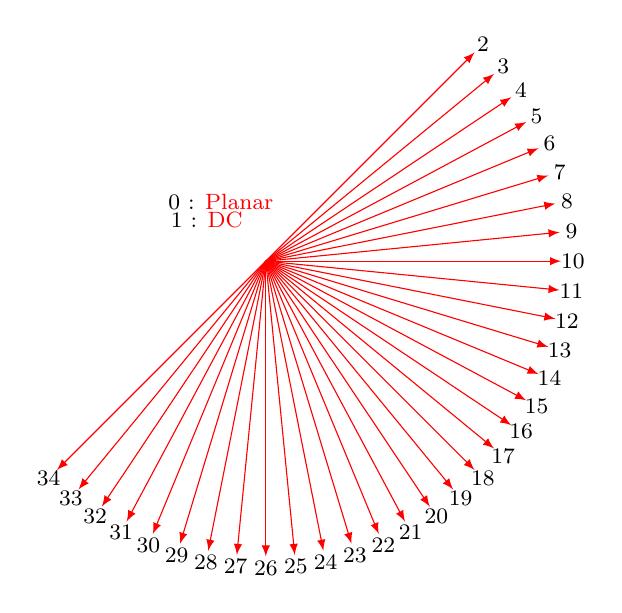
\begin{tikzpicture}[scale=1.5]

    \def\startx{0}
    \def\starty{0}
    \def\radius{2.5}
    \def\startangle{45}
    \def\colour{red}

    \draw (-0.38, 0.5) node {\footnotesize 0 : \color{red}{Planar}};
    \draw (-0.50, 0.5) node[below] {\footnotesize 1 : \color{red}{DC}};

    \foreach \direction in {2,3,...,34}
    {%
        % set the angle of current prediction direction 
        \pgfmathsetmacro{\angle}{\startangle - (\direction - 2) * 180 / 32}
        % horizontal directions (vertical scanning)
        \ifthenelse{\direction > 5 \AND \direction < 15}{\def\colour{blue}};
        % vertical directions (horizontal scanning)
        \ifthenelse{\direction > 21 \AND \direction < 31}{\def\colour{mygreen}};
        % draw the prediction direction lines with the appropriate colour
        \draw[-latex,\colour, thin] (\startx,\starty) --++ (\angle:\radius);
        % label each prediction direction
        \draw(\angle:\radius + 0.1) node {\footnotesize \direction};
    }

\end{tikzpicture}
